\clearpage

\section{SM and Higgs results}
\label{section_sm_higgs}

The Standard Model have been proven extremely successful in describing what it is proposed to do. The discovery of the two highest invariant mass particles of the SM, the top quark~\cite{top_discovery_cdf,top_discovery_d0}, by the CDF and 0 collaboration, at FERMILAB, and the Higgs Boson~\cite{higgs_discovery_cms,higgs_discovery_atlas}, by CMS and ATLAS, at CERN, fill the two missing pieces of the SM puzzle, presented at Figure~\ref{sm_summary}. In general, SM measurements presents very good agreement between theory and experiment, even when the Higgs boson is taken into account, once it mass has been established, the subsequent results tend to be found restricted within the expectations and constrained by the statistics and experimental sensitivity.  

In this section, we shall briefly review some of the most relevant SM results from LHC, with special focus to $Z$ and Higgs boson, subjects of the study. 

\subsection{Standard Model vector bosons resultsat CMS}
\label{section_sm_vb_results}

\begin{sidewaysfigure}[htbp]
  \centering
  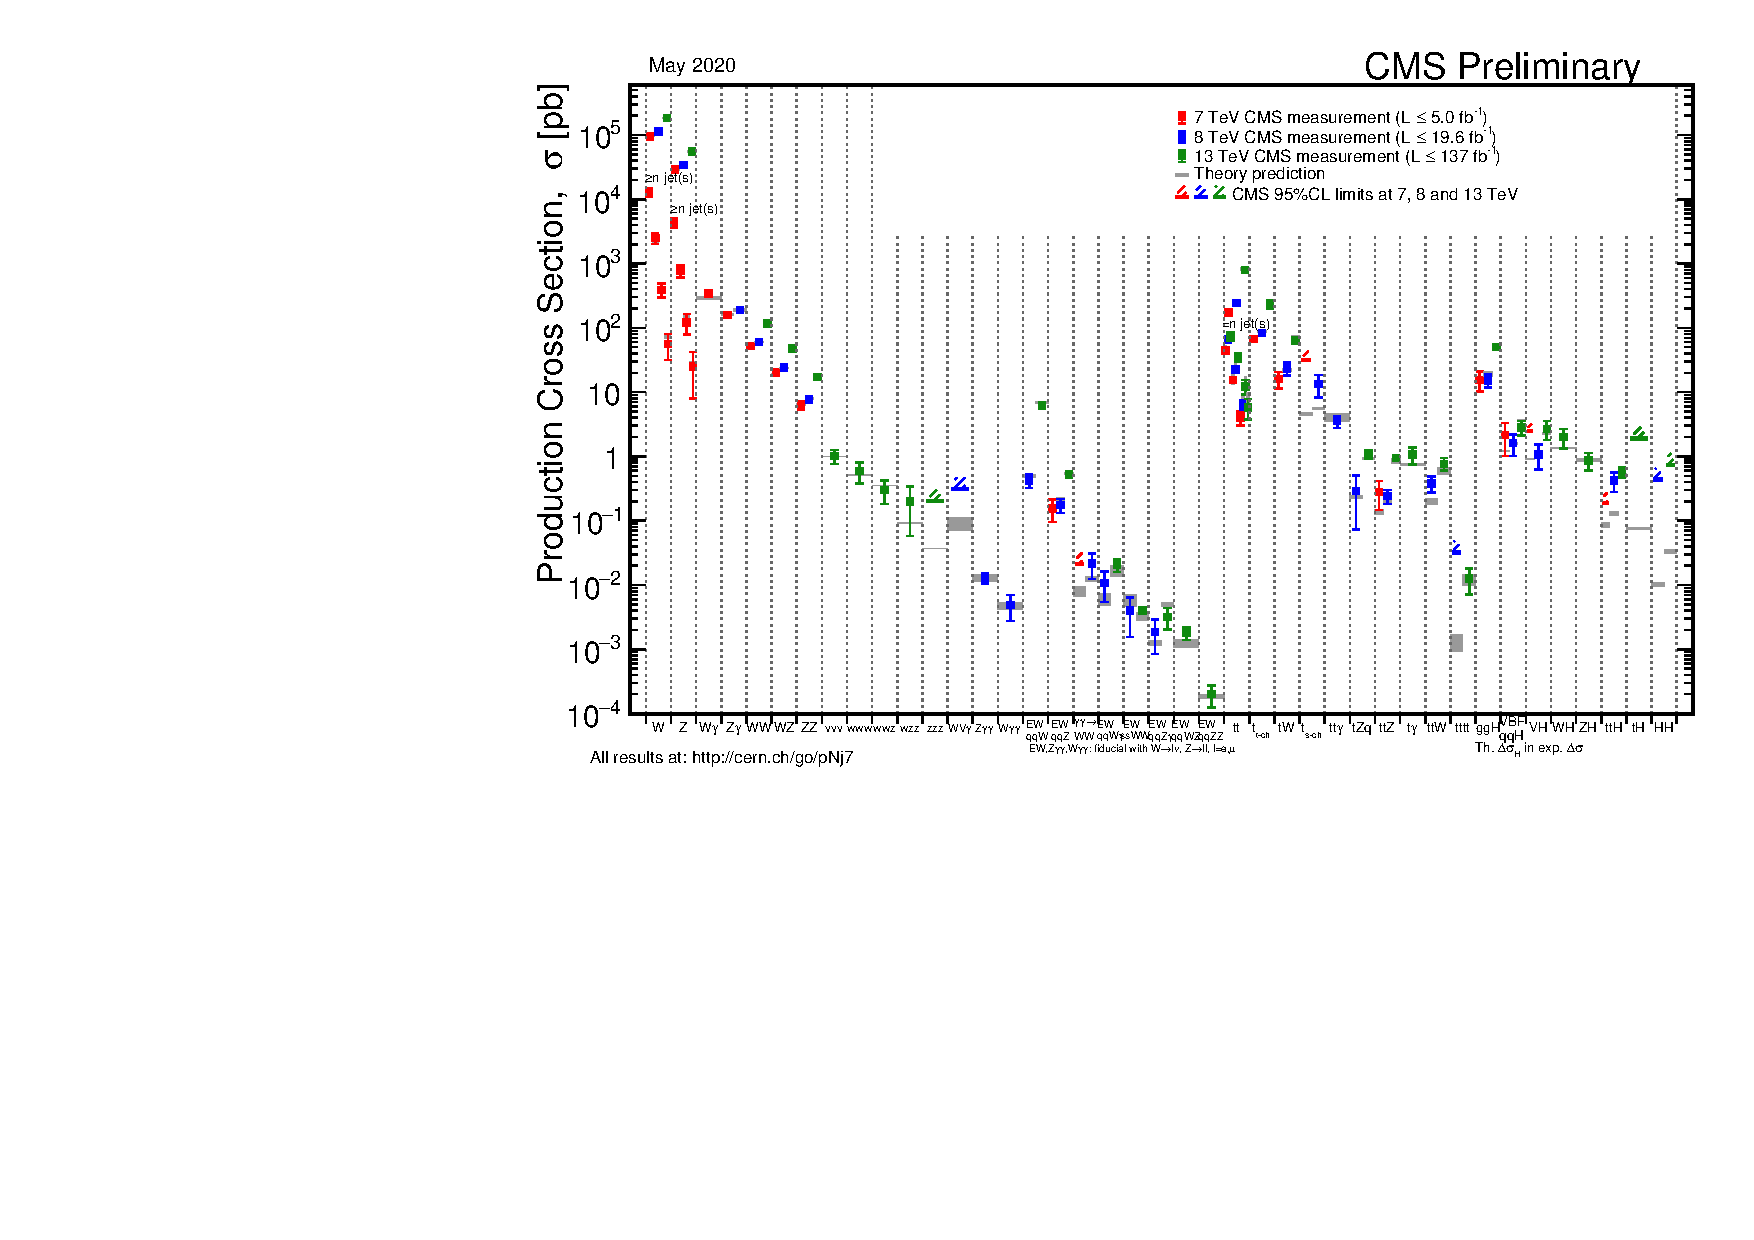
\includegraphics[width=\textwidth]{figures_and_tables/theory/cms_sm_xsec.pdf}
  \caption{\todo[inline]{SM x-sec!!!!!} Summary of the cross section measurements of Standard Model processes at CMS. Source:~\cite{cms_sm_xsec_summary}.}
  \label{cms_sm_xsec}
\end{sidewaysfigure}

\begin{figure}[htbp]
  \centering
  \begin{subfigure}[htbp]{0.48\textwidth}
    \centering
    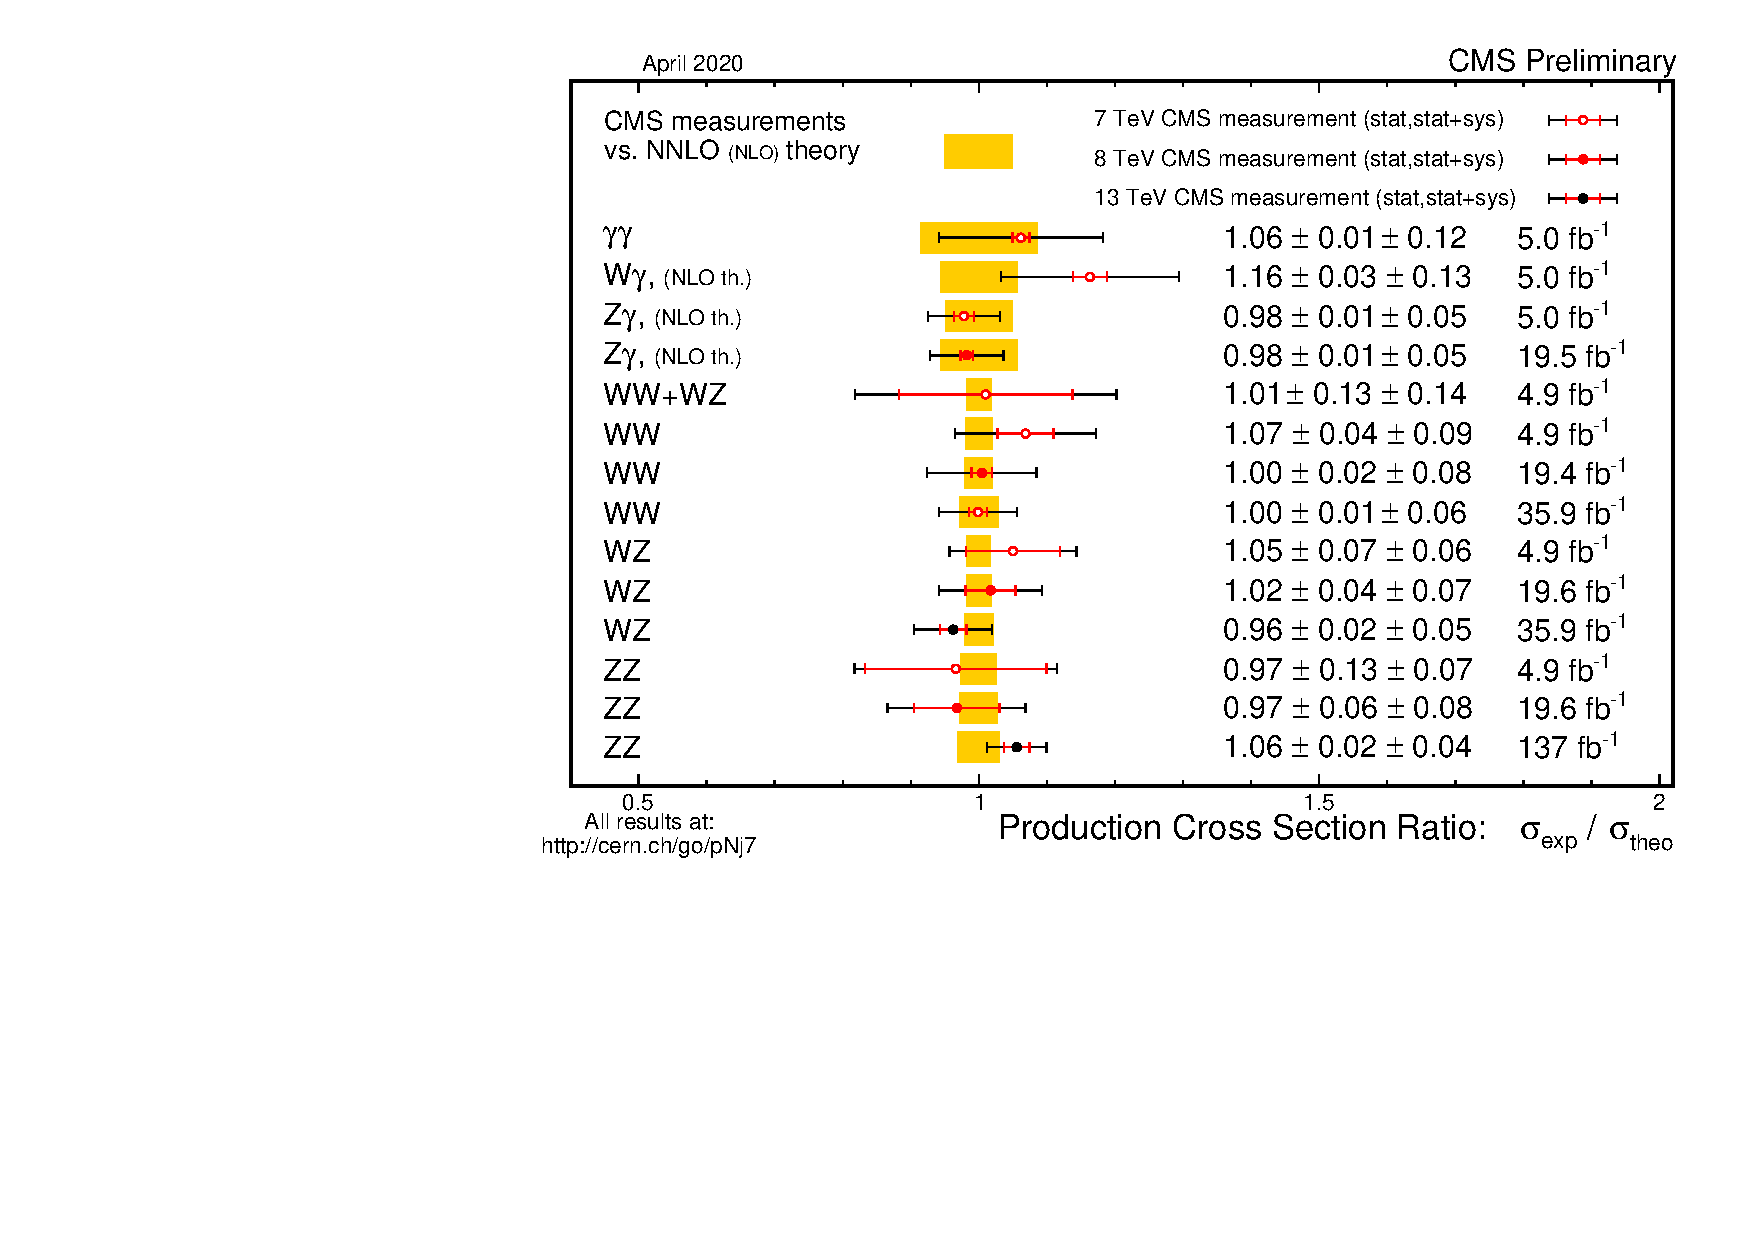
\includegraphics[width=\textwidth]{figures_and_tables/theory/sm_vbf_results.pdf}
    \caption{\todo[inline]{Expanadir!} Di-boson cross section ratio comparison to theory: Theory predictions updated to latest NNLO calculations where available compared to predictions in the CMS papers and preliminary physics analysis summaries. Source:~\cite{cms_sm_xsec_summary}.}
  \label{sm_vbf_results}
  \end{subfigure}
  \hfill
  \begin{subfigure}[htbp]{0.48\textwidth}
    \centering
    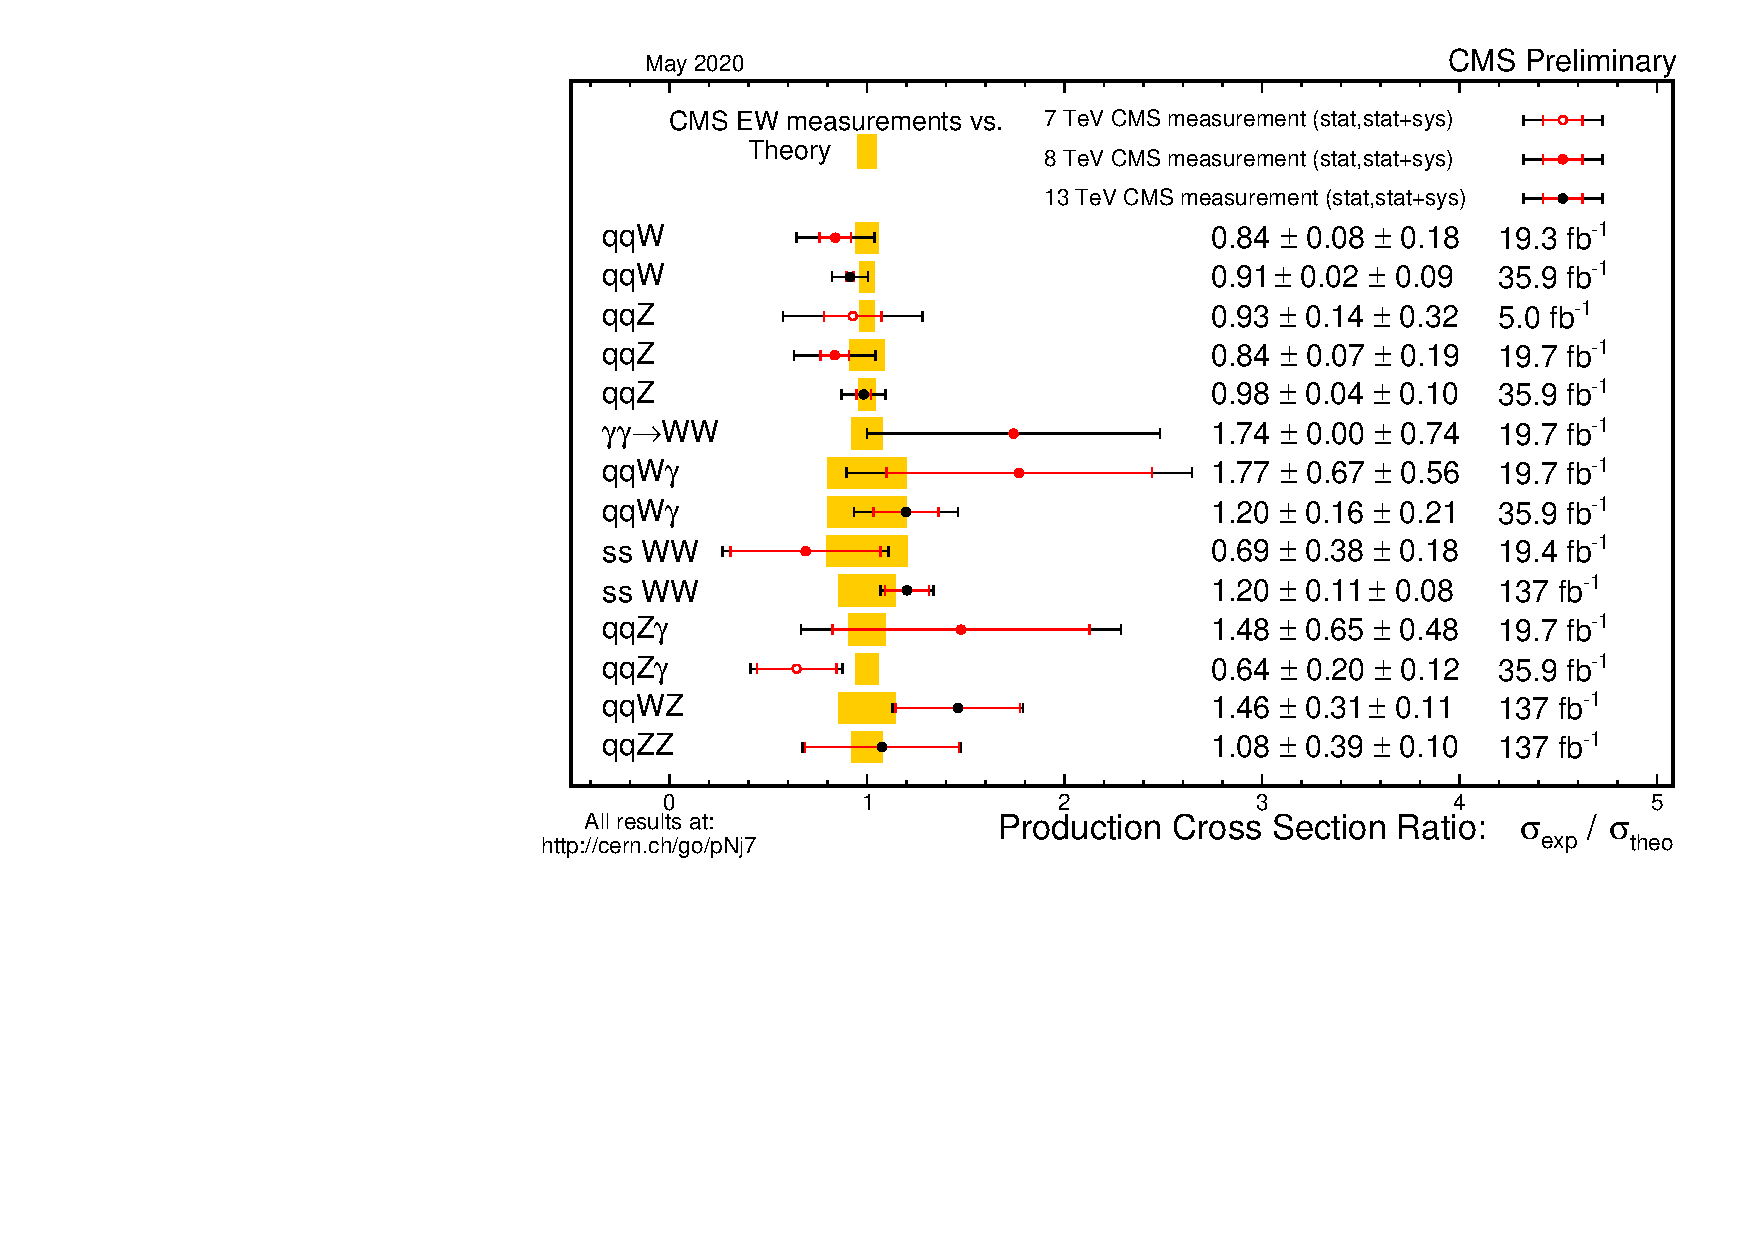
\includegraphics[width=\textwidth]{figures_and_tables/theory/sm_ewk_results.pdf}
    \caption{\todo[inline]{Expanadir!} Summary of the cross sections of pure Electroweak (EWK) interactions among the gauge bosons presented as a ratio compared to theory. Source:~\cite{cms_sm_xsec_summary}.}
    \label{sm_ewk_results}
  \end{subfigure}
\end{figure}

\subsection{Higgs boson results at CMS}
\label{section_sm_vb_results}

The Higgs may be produced at LHC proton-proton collisions by the following process, called \mbox{\textbf{production modes}}. Their SM expected cross section, as a function of the the Higgs mass is presented at Figure~\ref{higgs_prod_modes} and examples of leading order Feynmann diagrams are presented at Figure~\ref{fig_diagrams_production_modes}, for the highest cross section production modes.

The \textbf{Gluon Fusion - ggF} - is the result of a gluon-gluon interaction which is mediated by a heavy quark loop. Is by far the one with highest cross section. Its final state is composed only by a Higgs boson, which makes it harder to identify, since there are no other auxiliary final state particle to tag it. The \textbf{Associated Vector Boson Production - VH} - a SM vector boson (Z or W) irradiate a Higgs. Due to its clear electroweak signature (a final state with a Higgs and a vector boson), this production mode enhances the signal, when the Higgs decay has a large contribution from QCD background, e.g. $H \rightarrow b\bar{b}$. This process is also called Higgs-Strahlung.

The third process is the \textbf{Vector Boson Fusion - VBFH} - in which the two quarks from the initial state irradiate a pair of vector bosons (ZZ or $W{\pm}W{\mp}$). Those would interact (fuse) and produce a Higgs in the final, associated with two jets from the initial state quarks. The \textbf{Associated ttH Production - ttH} - and 
\textbf{Associated bbH Production - bbH} are very similar process (especially in the scale of $\sqrt{s} = 13$ TeV, where their cross sections almost match), where the coupling of the heavy quark to the Higgs boson, contrary to what happens in the ggF production, it is not with a virtual state of then. 

The \textbf{Associated Single Top Production - tH} - is the production mode with the smallest cross section, due to its destructive interference with other process. Without loss of generality, it is not considered in this study.


\begin{figure}[htbp]
  \centering
  \begin{subfigure}[htbp]{0.48\textwidth}
    \centering
    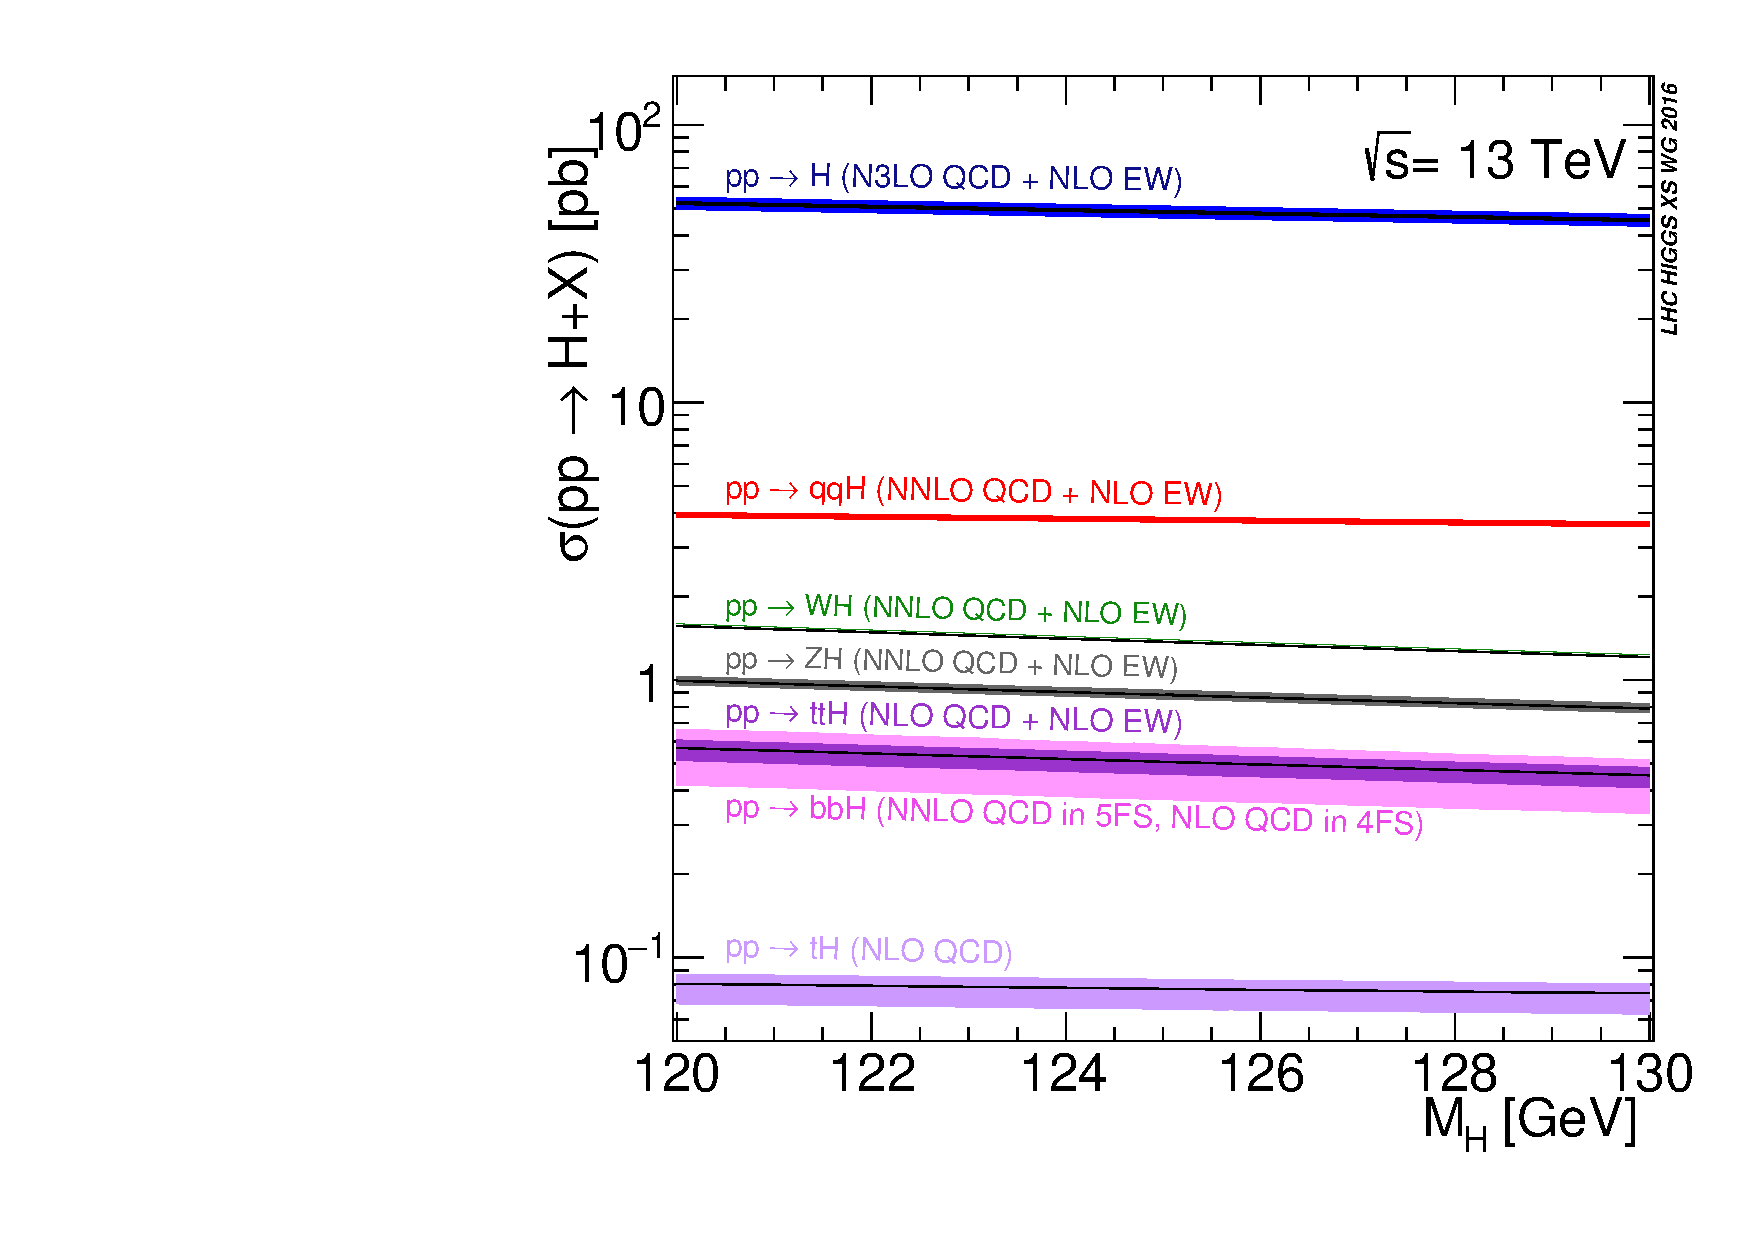
\includegraphics[width=\textwidth]{figures_and_tables/theory/higgs_prod_modes.pdf}
    \caption{\todo[inline]{Exapandir!}  Standard Model Higgs boson production cross sections at $\sqrt{s}=13$ TeV as a function of Higgs boson mass. The tH production cross section accounts for $t$-channel and $s$-channel only (no $tWH$ production). Source:~\cite{deFlorian:2016spz}.}
  \label{higgs_prod_modes}
  \end{subfigure}
  \hfill
  \begin{subfigure}[htbp]{0.48\textwidth}
    \centering
    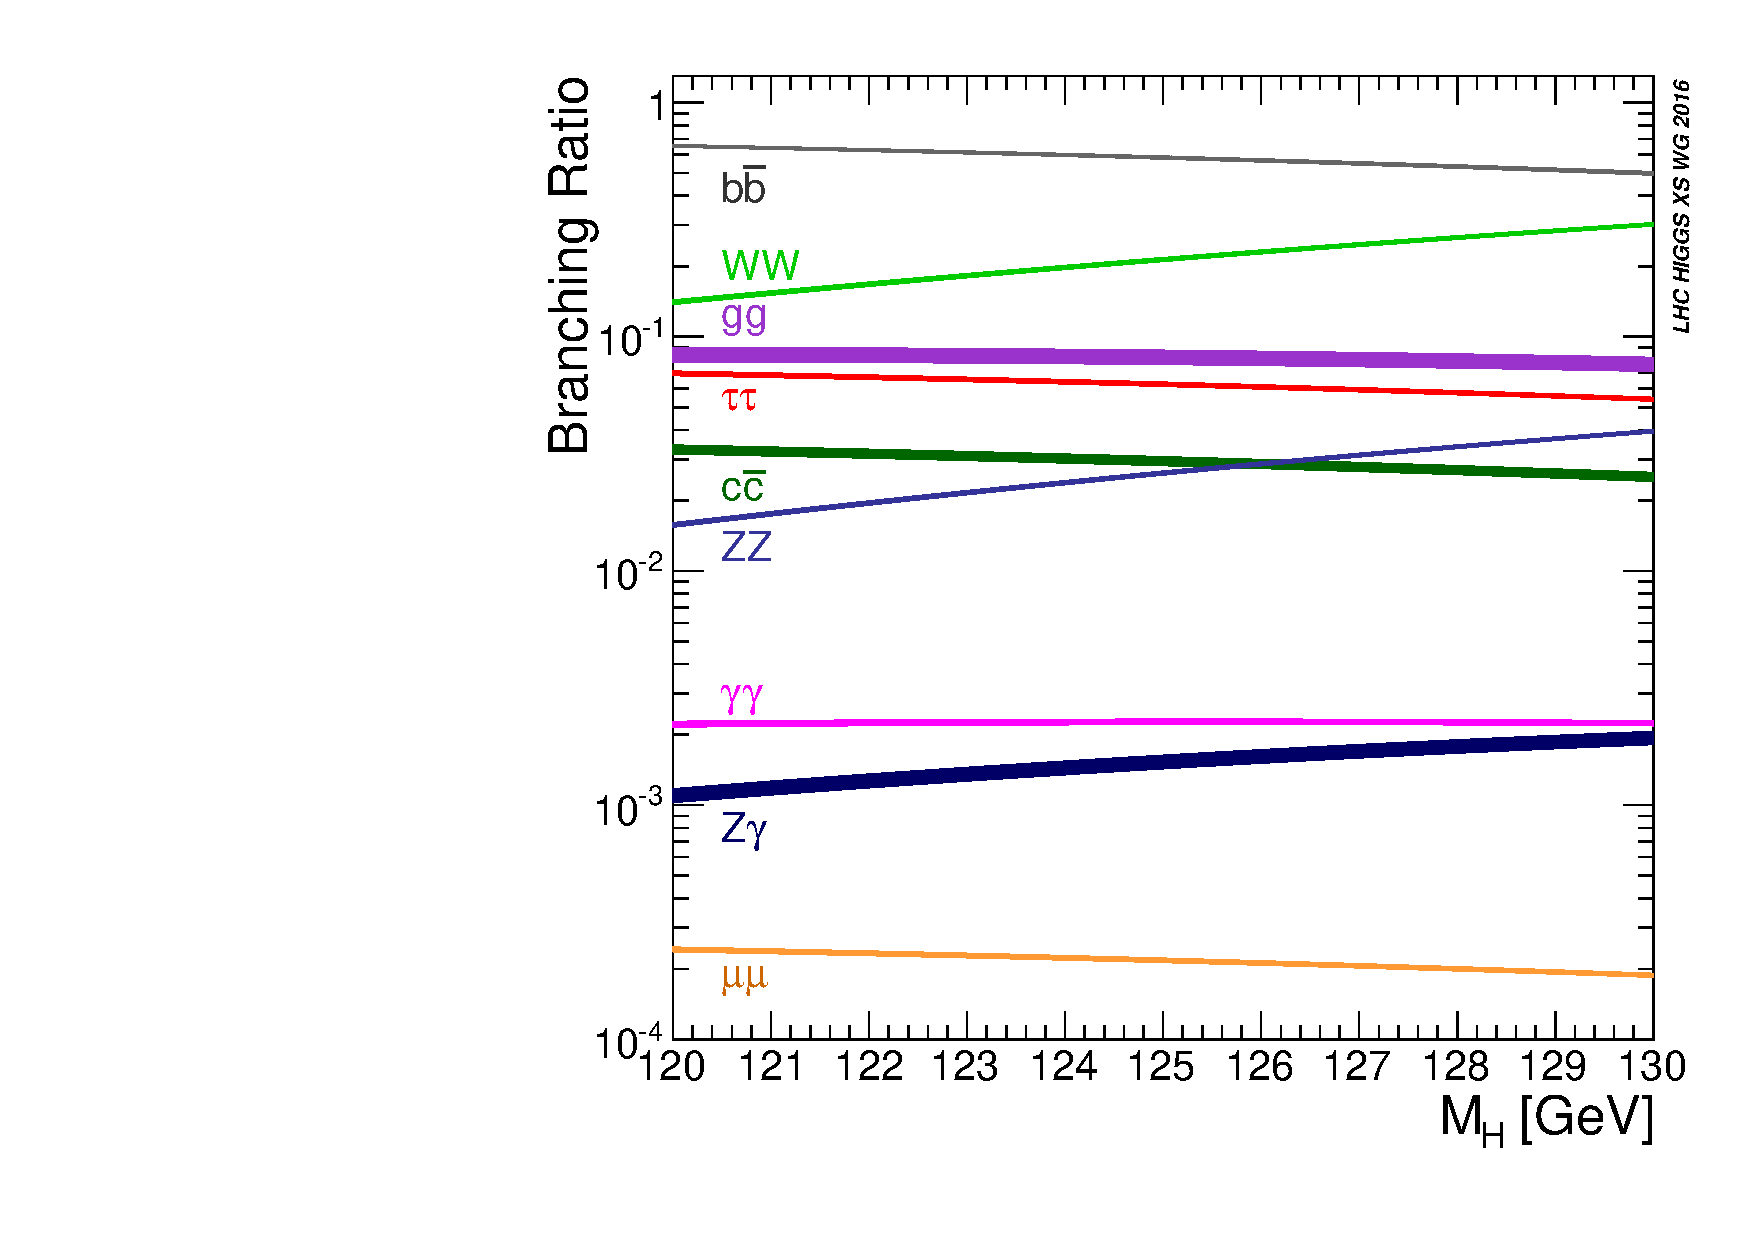
\includegraphics[width=\textwidth]{figures_and_tables/theory/higgs_decays.pdf}
    \caption{\todo[inline]{Exapandir!} Standard Model Higgs boson decay branching ratios for each decays channel. Source:~\cite{deFlorian:2016spz}.}
    \label{higgs_decays}
  \end{subfigure}
\end{figure}

% production modes
\begin{figure}[htbp]
  \centering
  \begin{subfigure}[htbp]{0.48\textwidth}
    \centering
    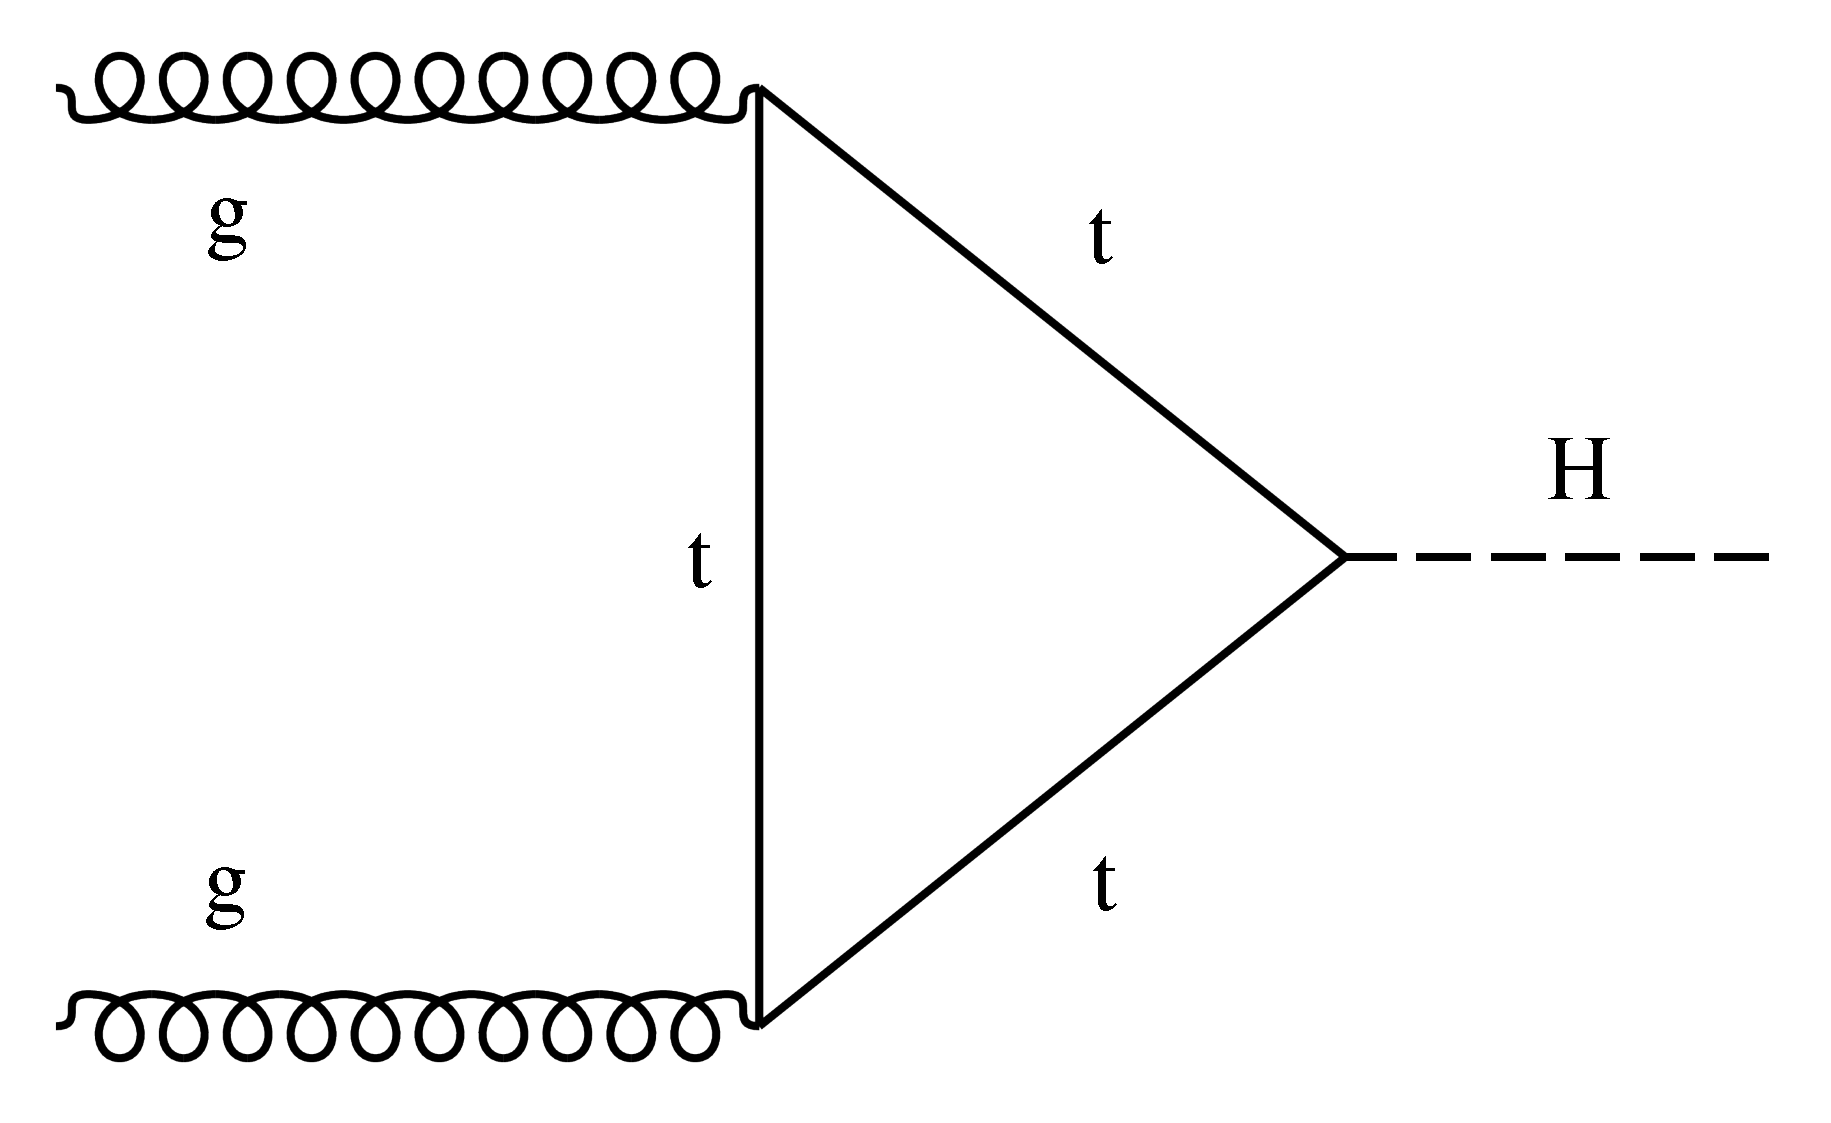
\includegraphics[width=\textwidth]{figures_and_tables/theory/higgs_prod_and_decays/ggf.pdf}
    \caption{Gluon Fusion - ggF}
  \end{subfigure}
  \hfill
  \begin{subfigure}[htbp]{0.48\textwidth}
    \centering
    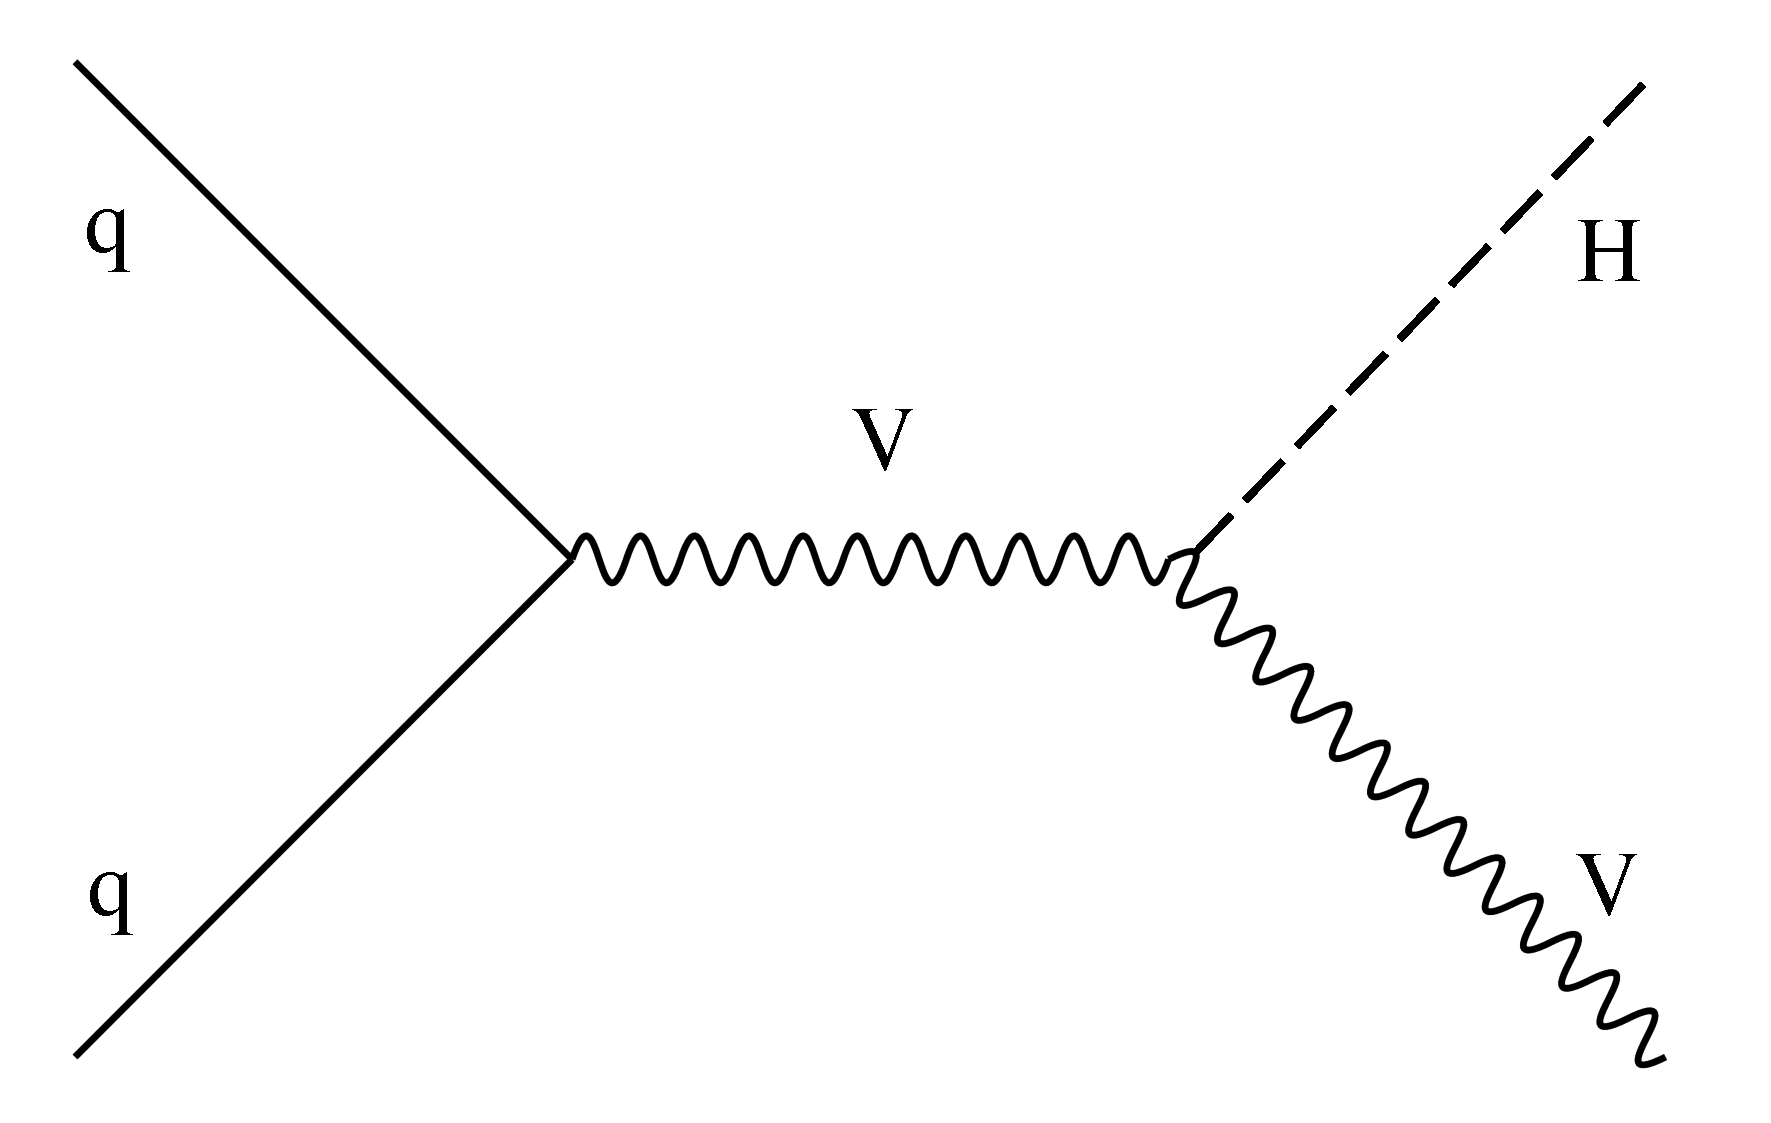
\includegraphics[width=\textwidth]{figures_and_tables/theory/higgs_prod_and_decays/vh.pdf}
    \caption{Associated Vector Boson Production - VH}
  \end{subfigure}
  \begin{subfigure}[htbp]{0.48\textwidth}
    \centering
    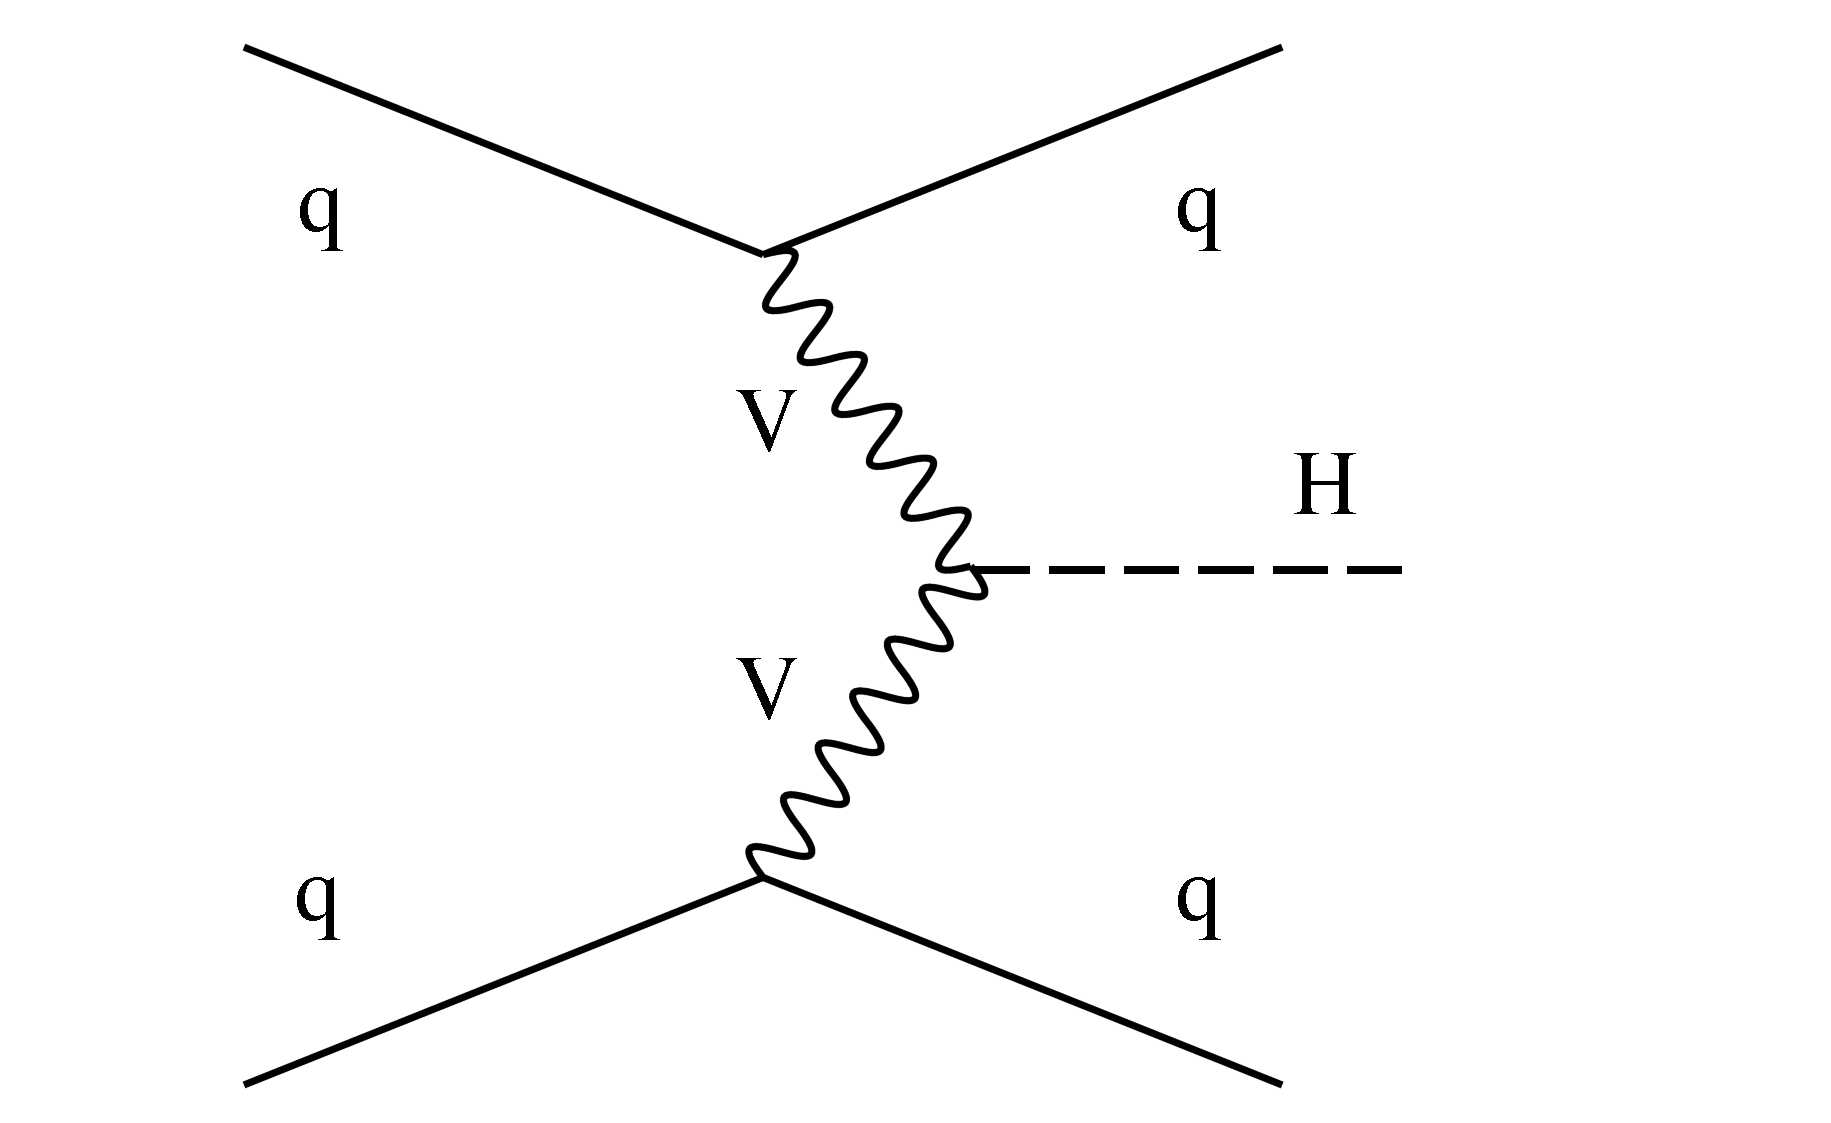
\includegraphics[width=\textwidth]{figures_and_tables/theory/higgs_prod_and_decays/vbf.pdf}
    \caption{Vector Boson Fusion - VBFH}
  \end{subfigure}
  \hfill
  \begin{subfigure}[htbp]{0.48\textwidth}
    \centering
    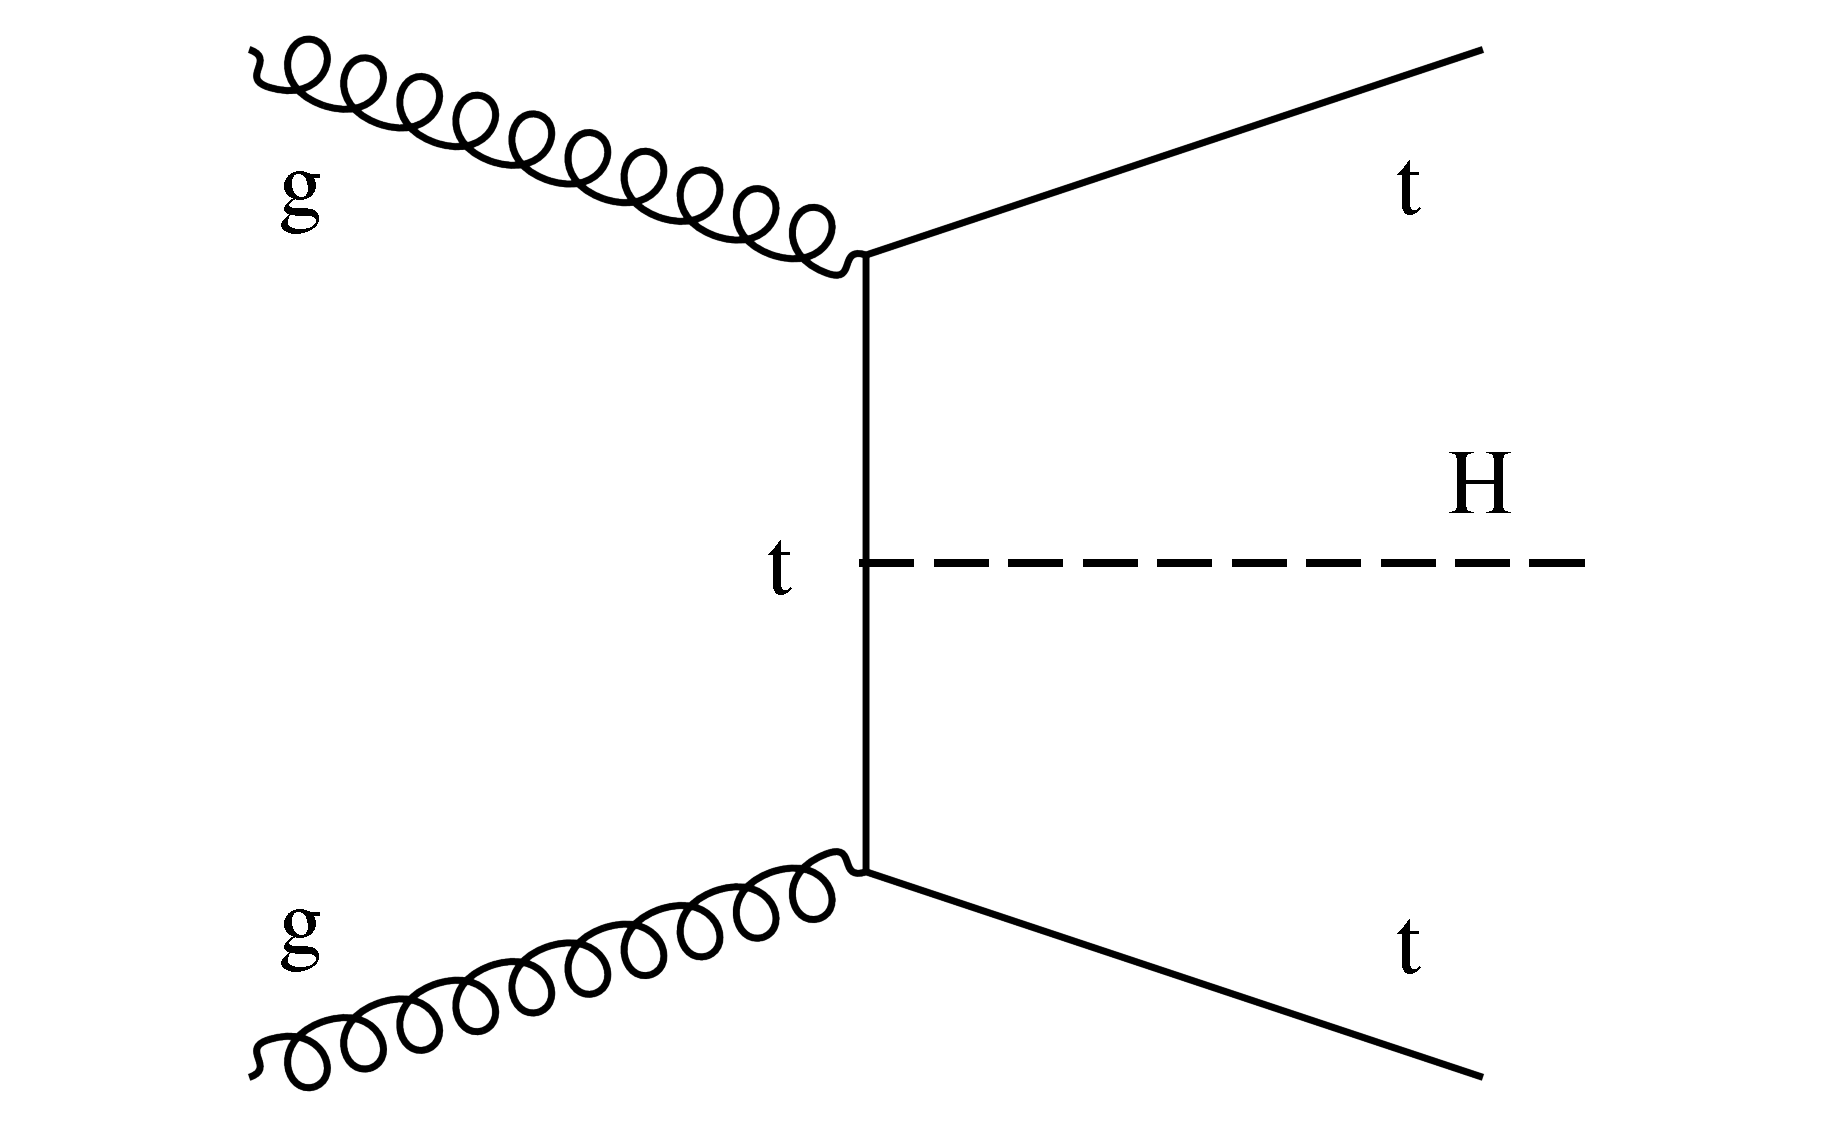
\includegraphics[width=\textwidth]{figures_and_tables/theory/higgs_prod_and_decays/tth.pdf}
    \caption{Associated ttH Production - ttH}
  \end{subfigure}
  \caption{\todo[inline]{Exapandir!} Example of leading order Standard Model Higgs boson production model diagrams. Source:~\cite{higgs_diagrams}.}
  \label{fig_diagrams_production_modes}
\end{figure}



As already mentioned on Section~\ref{section_sm_higgs}), the Higgs have been found at CMS and ATLAS in 2012, by investigating 


% Higgs discovery
\begin{figure}[htbp]
  \centering
  \begin{subfigure}[htbp]{0.48\textwidth}
    \centering
    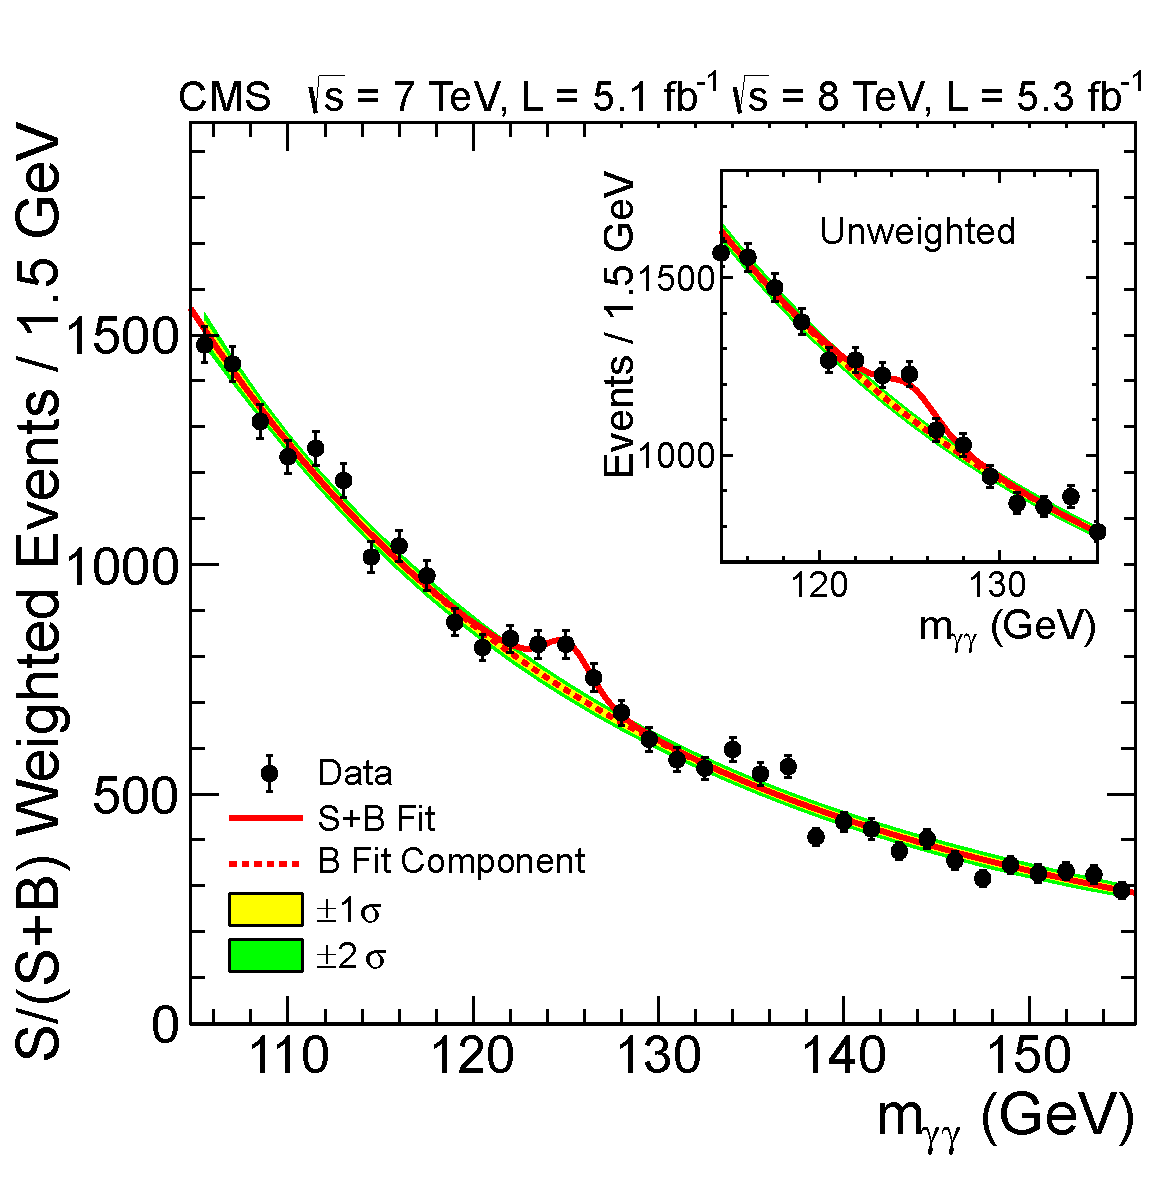
\includegraphics[width=\textwidth]{figures_and_tables/theory/higgs_discovery_hgg.pdf}
    \caption{\todo[inline]{Exapandir!} The diphoton invariant-mass distribution for the 7 and 8 \TeV datasets (points), with each event weighted by the predicted $S/(S+B)$ ratio of its event class. The solid and dotted lines give the results of the signal-plus-background and background-only fit, respectively. The light and dark bands represent the $\pm$1 and $\pm$2 standard deviation uncertainties respectively on the background estimate. The inset shows the corresponding unweighted invariant-mass distribution around \mbox{$m_{\gamma\gamma}$ = 125 \GeV}. Source:~\cite{higgs_discovery_cms}.}
  \label{higgs_discovery_hgg}
  \end{subfigure}
  \hfill
  \begin{subfigure}[htbp]{0.48\textwidth}
    \centering
    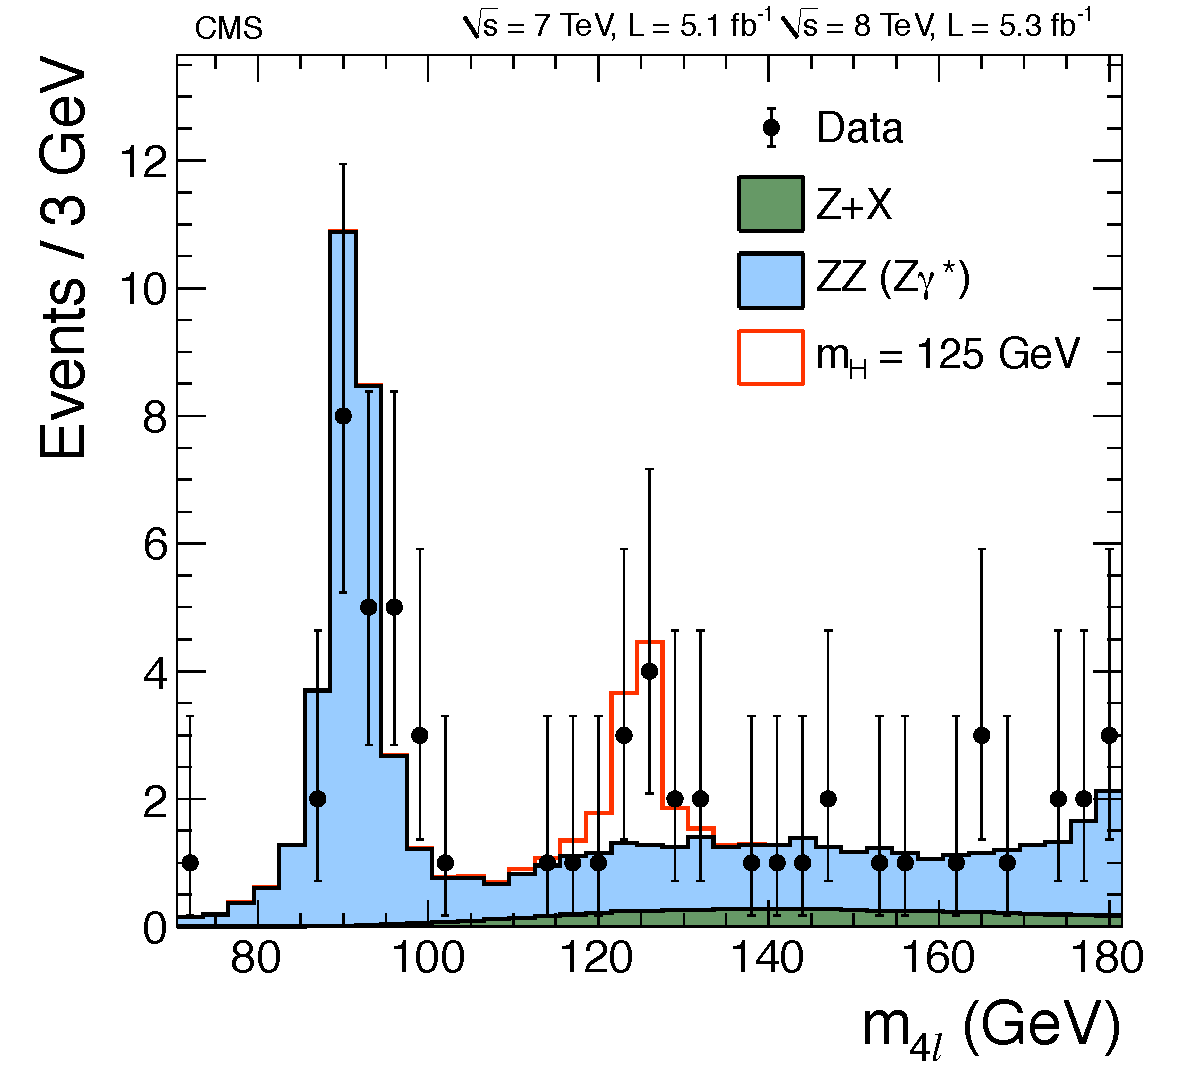
\includegraphics[width=\textwidth]{figures_and_tables/theory/higgs_discovery_hzz4l.pdf}
    \caption{\todo[inline]{Exapandir!} Distribution of the observed four-lepton invariant mass from the combined 7 and 8 \TeV data 
    for the $\PH \to \cPZ\cPZ\to 4\ell$ analysis (points).
    The prediction for the expected $\cPZ$+X and $\cPZ\cPZ(\cPZ\gamma^*)$ background are shown by the dark and light histogram, respectively. The open histogram gives the expected distribution for a Higgs boson of mass 125 \GeV. Source:~\cite{higgs_discovery_cms}.}
    \label{higgs_discovery_hzz4l}
  \end{subfigure}
\end{figure}


\todo[inline]{discovery}
\todo[inline]{Production modes}
\todo[inline]{Decay modes}


\todo[inline]{Yukawa coupling}

\todo[inline]{Higgs results at CMS}






% signal strength modifier - COMB RUn2
\begin{figure}[htbp]
  \centering
  \begin{subfigure}[htbp]{0.48\textwidth}
    \centering
    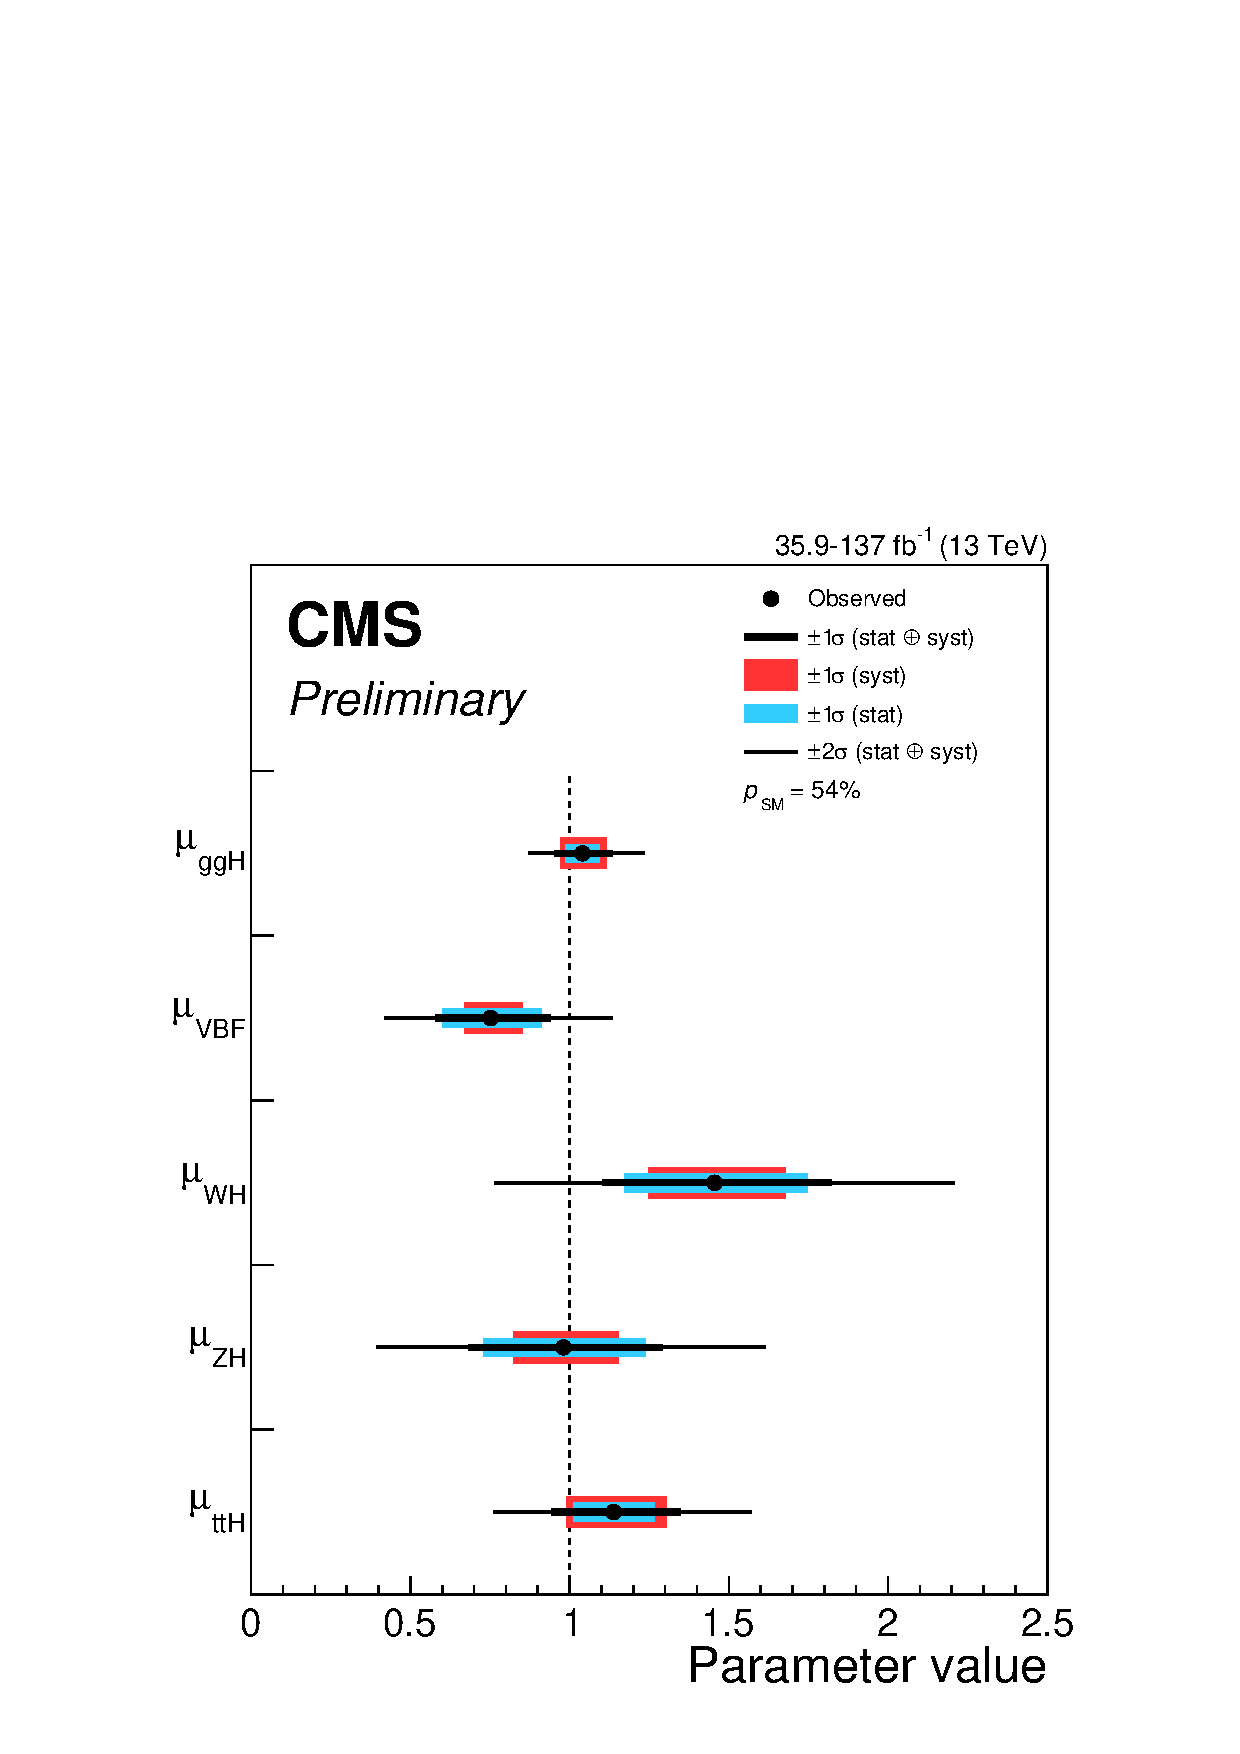
\includegraphics[width=\textwidth]{figures_and_tables/theory/signal_strength_modifier_prod.pdf}
    \caption{ }
  \label{signal_strength_modifier_prod}
  \end{subfigure}
  \hfill
  \begin{subfigure}[htbp]{0.48\textwidth}
    \centering
    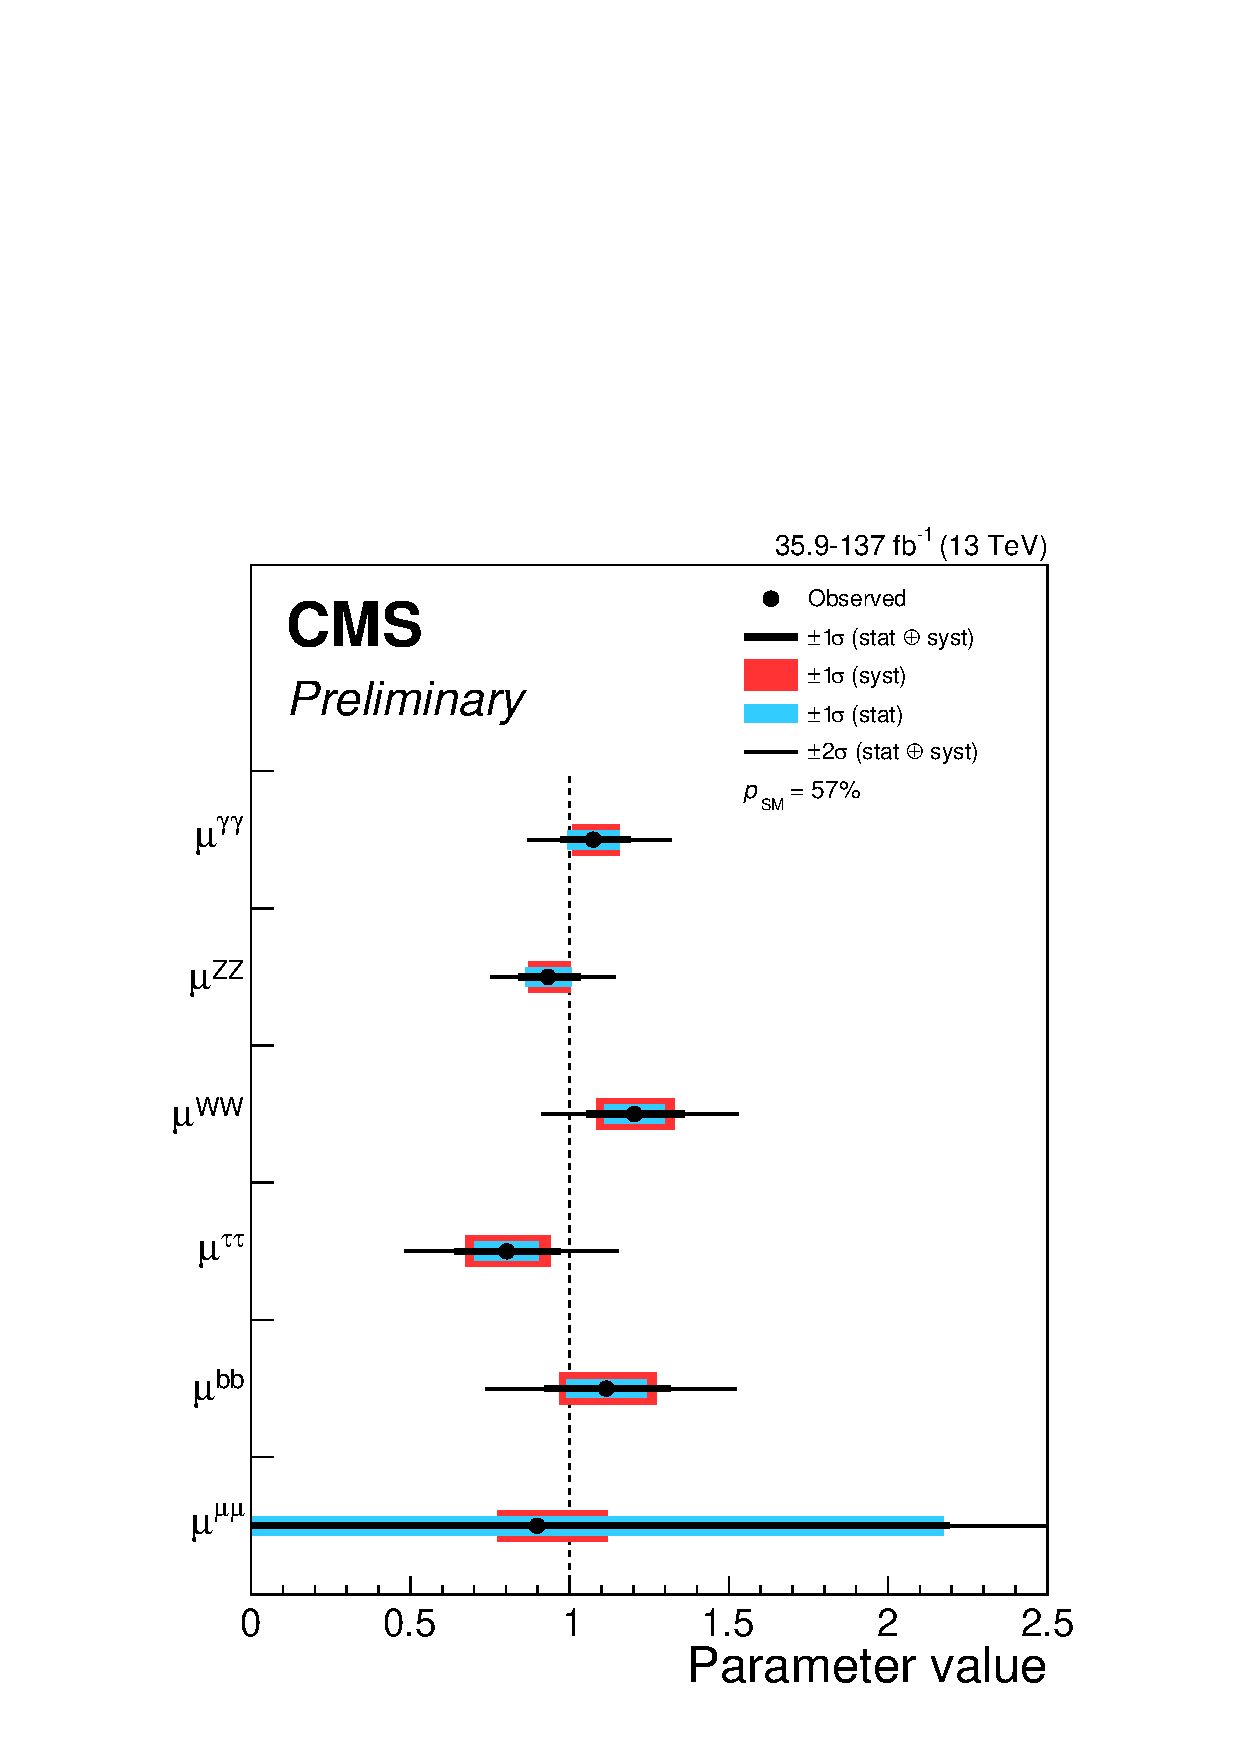
\includegraphics[width=\textwidth]{figures_and_tables/theory/signal_strength_modifier_decay.pdf}
    \caption{ }
    \label{signal_strength_modifier_decay}
  \end{subfigure}
  \caption{\todo[inline]{Expandir!} Signal strength modifiers for the production, $\mu^{i}$, and for the decay, $\mu^{f}$, modes on the left and the right panel, respectively. The thick (thin) black lines report the $1\sigma$ ($2\sigma$) confidence intervals. The thick blue and red lines report the statistical and systematic components of the $1\sigma$ confidence intervals. The assumptions used in this fit are described in the text. Source:~\cite{cms_higgs_comb_run2}.}
\end{figure}





% H to mumu
\begin{figure}[htbp]
  \centering
  \begin{subfigure}[htbp]{0.48\textwidth}
    \centering
    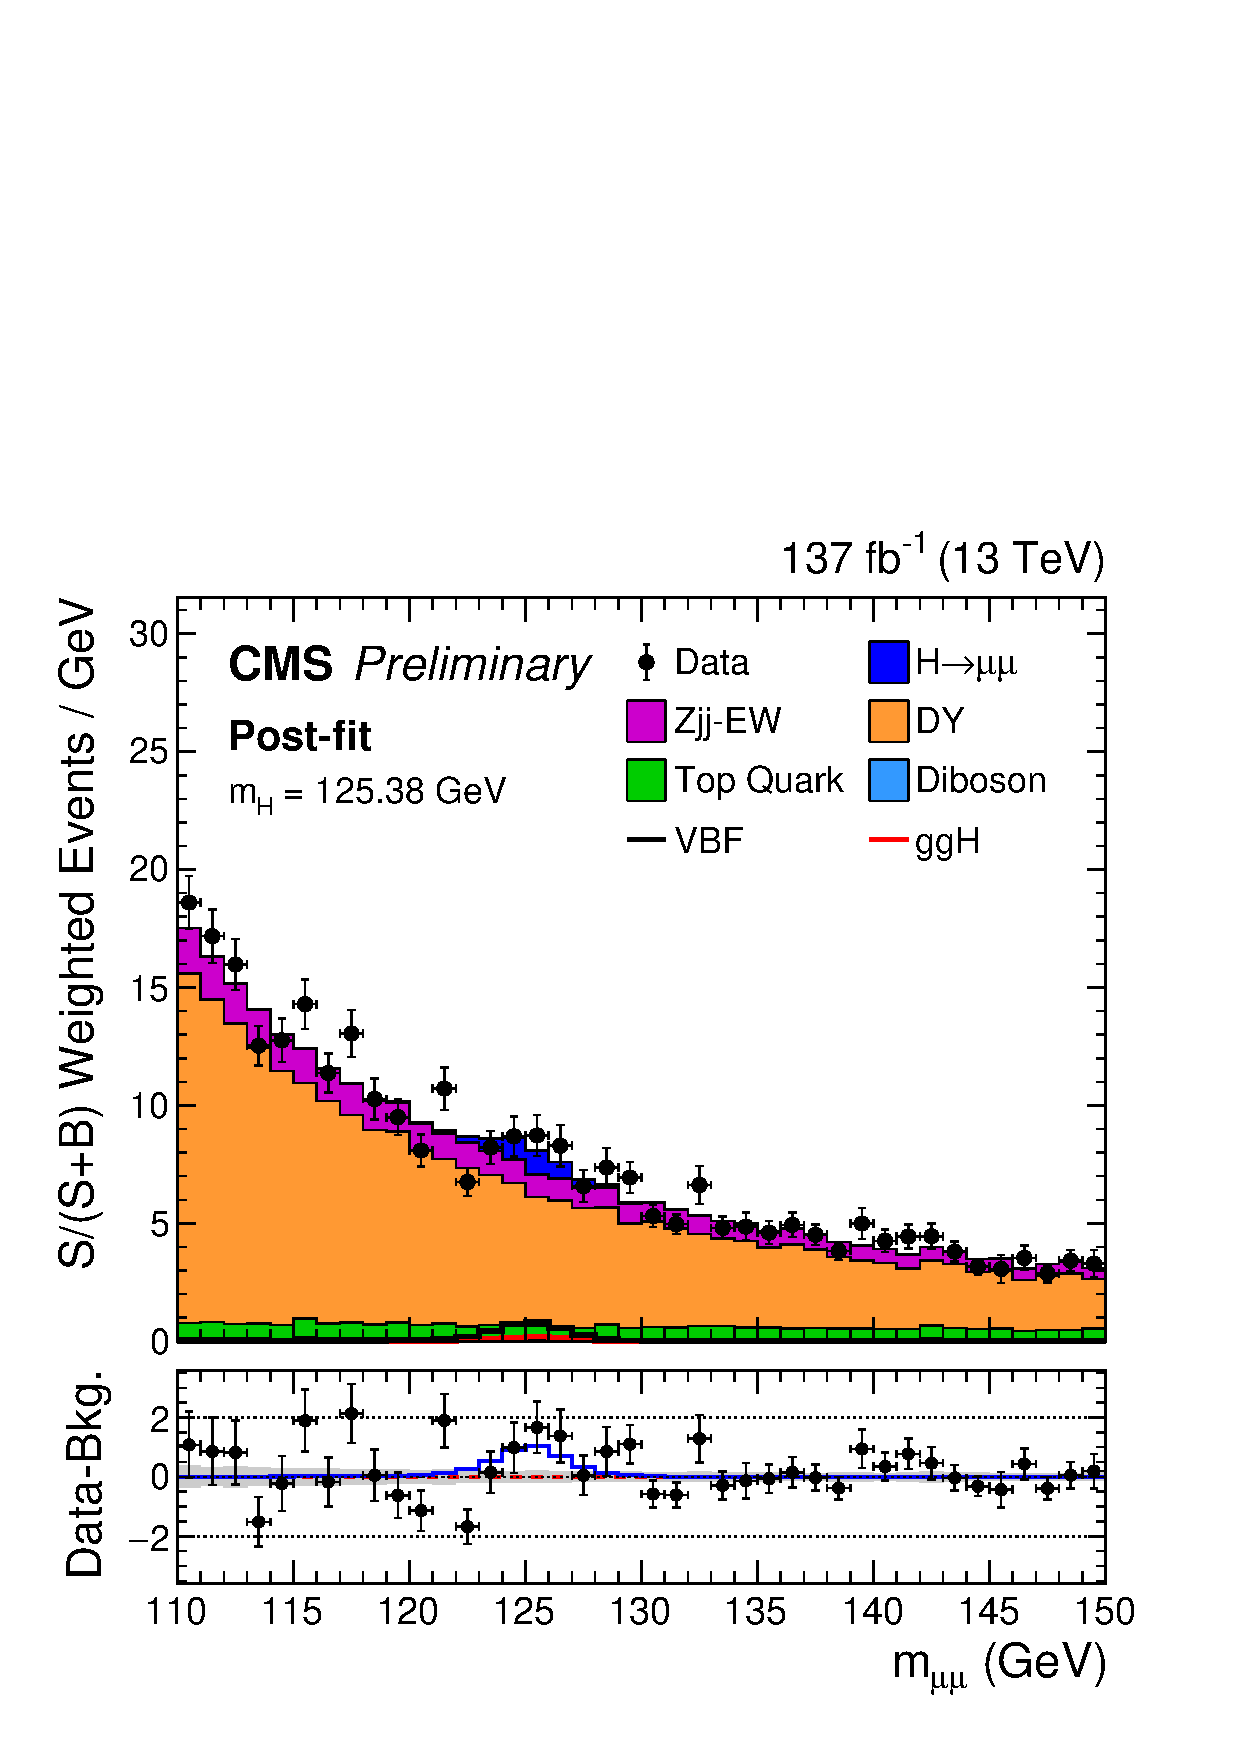
\includegraphics[width=\textwidth]{figures_and_tables/theory/h_to_mumu_result.pdf}
    \caption{\todo[inline]{Higgs to MuMu. É apenas um evidência!} The $m_{\mu\mu}$ distribution for the weighted combination of VBF events. Each event is weighted proportionally to the $S/(S + B)$ ratio. The lower panel shows the residuals after subtracting the background prediction from the signal-plus-background fit. The best-fit $H \rightarrow \mu\mu$ signal contribution is indicated by the blue line, and the grey band indicates the total background uncertainty from the background-only fit. The measured signal strength is ${1.19^{+0.41}_{-0.39}(\mathrm{stat})^{+0.17}_{-0.16}(\mathrm{sys})}$. Source:~\cite{cms_higgs_mumu}.}
  \label{h_to_mumu_result}
  \end{subfigure}
  \hfill
  \begin{subfigure}[htbp]{0.48\textwidth}
    \centering
    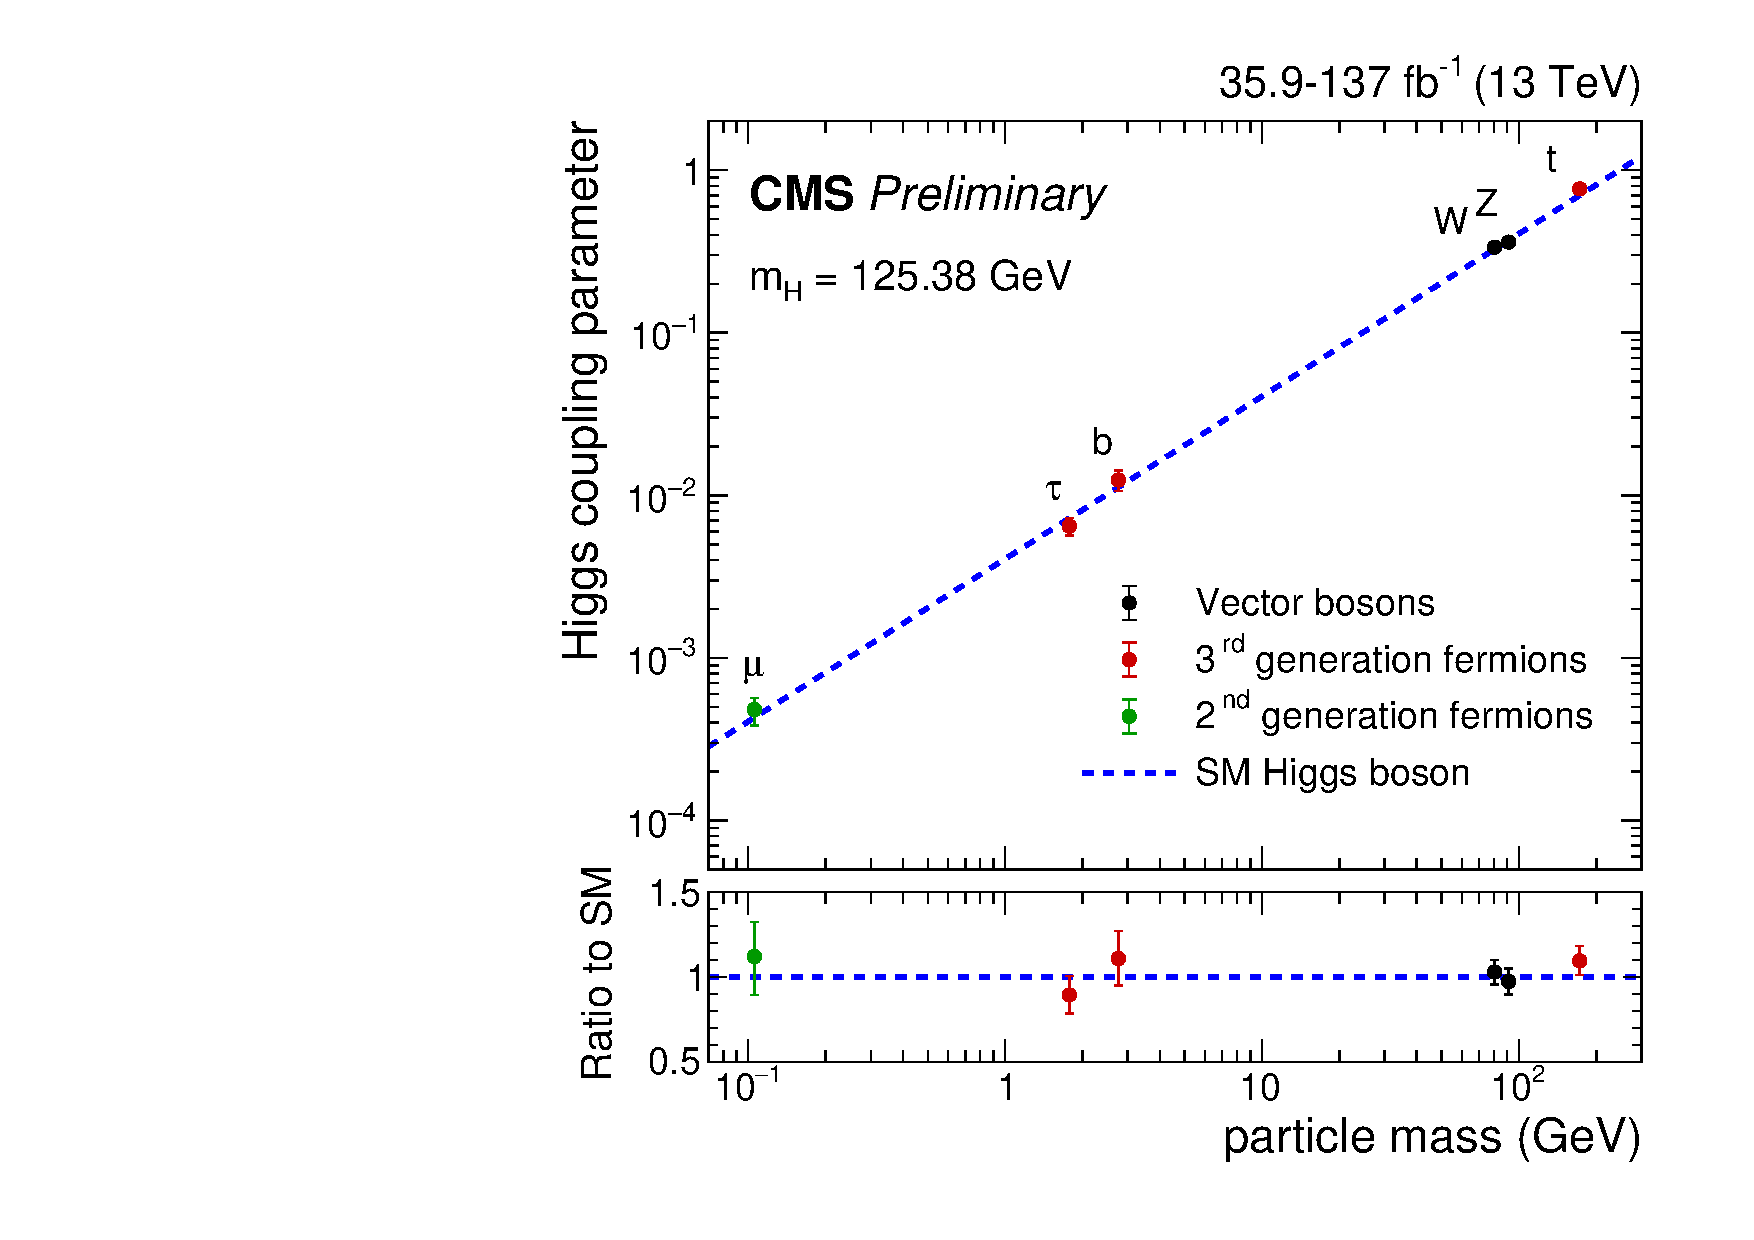
\includegraphics[width=\textwidth]{figures_and_tables/theory/higgs_coups.pdf}
    \caption{\todo[inline]{Higgs to MuMu. É apenas um evidência!} The best-fit estimates for the reduced coupling modifiers extracted for fermions and weak bosons from the resolved $\kappa$-framework model compared to their corresponding prediction from the SM. The error bars represent 68\% CL intervals for the measured parameters. The lower panel shows the ratios of the measured coupling modifiers values to their SM predictions. Source:~\cite{cms_higgs_mumu}.}
    \label{higgs_coups}
  \end{subfigure}
\end{figure}

